\subsection{Детерминированные и недетерминированные конечные автоматы, их эквивалентность. Минимизация ДКА.}
\D{
	Формально КА определяется как пятёрка:
	
	$A=(S,X,Y,\delta ,\lambda )$
	
	где 
	\begin{itemize}
		\item $S$ — конечное множество состояний автомата
		\item $X,Y$ — конечные входной и выходной алфавиты соответственно, из которых формируются строки, считываемые и выдаваемые автоматом
		\item $\delta :S\times X\rightarrow S$ — функция переходов
	 	\item $\lambda :S\times X\rightarrow Y$ — функция выходов
	\end{itemize}

	Можно добавить $s_0 \in S$ - начальное состояние.
	
	При анализе КА принято полагать, что конечный автомат начинает работу в некотором начальном состоянии $q_{0}$, последовательно получает по одному символу из входного слова (цепочки входных символов). Считанный символ может перевести автомат в новое состояние или не перевести в новое состояние в соответствии с функцией переходов.
	
	Получая входную цепочку символов $x$ и делая переходы из состояния в состояние, автомат после получения последнего символа входного слова окажется в некотором состоянии $q'$.
	
	Если это состояние является заключительным, то говорят, что автомат допустил слово $x$.
	
	Автомат называется конечным в силу конечности множества внутренних состояний.
}

Различают детерминированные КА — автоматы, в которых следующее состояние однозначно определяется текущим состоянием и выход зависит только от текущего состояния и текущего входа, и недетерминированные КА, следующее состояние у которых в общем случае неопределённо и, соответственно, не определён выходной сигнал. Если переход в последующие состояния происходит с некоторыми вероятностями, то такой КА называют вероятностным КА. 

\begin{figure}[H]
	\centering
	\begin{minipage}[b]{0.4\textwidth}
		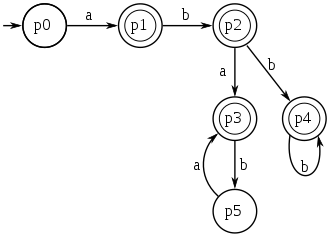
\includegraphics[width=\textwidth]{images/dfa.png}
		\caption{Пример графа переходов детерминированного КА.}
	\end{minipage}
	\hfill
	\begin{minipage}[b]{0.4\textwidth}
		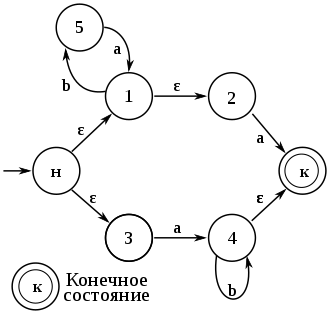
\includegraphics[width=\textwidth]{images/ndfa.png}
		\caption{Пример графа переходов недетерминированного КА с самопроизвольными переходами.}
	\end{minipage}
\end{figure}

\begin{itemize}
	\item Детерминированным конечным автоматом (ДКА) называется такой автомат, в котором нет дуг с меткой $\varepsilon$ (предложение, не содержащее ни одного символа), и из любого состояния по любому символу возможен переход не более, чем в одно состояние
	\item Недетерминированный конечный автомат (НКА) является обобщением детерминированного. Недетерминированность автоматов может достигаться двумя способами: либо могут существовать переходы из состояния в состояние, вызываемые пустой цепочкой символов, то есть самопроизвольные переходы без внешних воздействий, либо из одного состояния КА может переходить в разные состояния под воздействием одного и того же символа.
	
	Также недетерменированность может достигаться за счет не единственного (а множества) начальных состояний.
\end{itemize}

\D{
	Говорят, что детерменированный автомат принимает слово, если обработав его, он приходит в специальное конечное состояние. 
	
	Недетерменированный принимает, если \underline{существует} последовательность, такая что принимает.
}

\D{
	Язык автомата - множество принимаемых слов.
}

\T[О детерминизации]{
	Для любого недетрменированного конечного автомата может быть построен эквивалентный (с тем же языком) детерменированный автомат. 
}
\begin{proof}
	План:
	\begin{enumerate}
		\item Удалить все $\varepsilon$-переходы
		\begin{enumerate}[a]
			\item Удалить все состояния, в которые приходят только $\varepsilon$-ребра
			\item Соединить напрямую $p \rightarrow_a q$, если есть путь $p \rightsquigarrow_\varepsilon r \rightarrow_a q$
			\item Конечными делаем те состояния, из которых достижимы конечные по $\varepsilon$-ребрам
		\end{enumerate}
		\item Делаем исходящую степень $\leq 1$.
		
		Для этого множеством новых состояний положим множество всех подмножеств старых состояний. 
		
		Функция переходов нового конечного автомата определена так, что из состояния-множества $S$ по входному символу $а$ конечный автомат $M_1$ переходит в состояние-множество, представляющее собой объединение всех множеств состояний старого конечного автомата, в которые этот старый конечный автомат переходит по символу $а$ из каждого состояния множества $S$. Таким образом, конечный автомат $M_1$ является детерминированным по построению.
	\end{enumerate}

	Более подробно:  \href{http://mathhelpplanet.com/static.php?p=determinizatsiya-konechnykh-avtomatov}{Доказательство}.
	
	Заметим, что размер автомата может раздуться экспоненциально. 
\end{proof}

\subsubsection{Минимизация ДКА}

Минимизация ДКА — построение по детерминированному конечному автомату (ДКА) эквивалентного ДКА, имеющего наименьшее возможное число состояний. 

\T{
	Для любого регулярного языка существует минимальный ДКА, который его принимает, то есть, ДКА с наименьшим возможным числом состояний. Такой автомат единственен с точностью до изоморфизма. 
}

А вот дальше реально прикол, готовьтесь
\T{
	Пусть $\mathcal {A}$ — ДКА. Обозначим через $r({\mathcal {A}})$ инвертированный автомат $\mathcal {A}$. Через  $d({\mathcal {A}})$ обозначим детерминизированный автомат, полученный из $\mathcal {A}$ процедурой построения подмножеств. Имеет место следующий результат:
	
	Пусть автомат $\mathcal {A}$ распознаёт язык $L$. Тогда минимальный ДКА для языка $L$ может быть найден как $\mathcal {A}_{L}=drdr({\mathcal {A}})$.
}

\subsubsection{Регулярные языки}
\D{
	Пусть $\Sigma$ - конечный алфавит. Регулярными языками над $\Sigma$ называются языки, получаемые по следующим правилам:
	\begin{enumerate}
		\item Пустое множество - регулярный язык
		\item Множество, состоящие из пустой строки - регулярный язык
		\item Множество вида $\{a\}, a \in \Sigma$ - регулярный язык
		\item Если $\alpha, \beta$ - регулярные языки, то 
		\begin{itemize}
			\item $\alpha \cup \beta$
			\item Конкатенация $\alpha\beta$
			\item Взятие звездочки Клини $\alpha^*$
		\end{itemize}
		 - регулярные языки, где
		 
		 Звезда Клини языка $\alpha$ - минимальное множество слов, полученых конкатенацией слов из $\alpha$ и пустой строки. 
	\end{enumerate}
}

\T[Клини]{
	Язык является регулярным тогда и только тогда, когда он допускается некоторым конечным автоматом, используемым в этом языке. 
}